\documentclass{template}
\usepackage{graphicx,parskip,appendix,float, subcaption}
\usepackage{fancyhdr, lastpage}
\usepackage[ruled] {algorithm2e}
\usepackage{url,amsmath,amssymb,fancybox,listings,pdfpages,caption,multicol,datetime,rotating, booktabs, minted, epigraph}
%\usepackage[usenames,dvipsnames]{color}
\usepackage[pagebackref=false,pdffitwindow=true]{hyperref}
\usepackage{csquotes}
\usepackage[style=numeric,backend=biber]{biblatex}
\graphicspath{{./images}}
\addbibresource{library.bib}

%NOTE: The hyperref usepackage should be the last \usepackage!!
%NOTE: When pagebackref=true an error will appear at the end of compiling. press `q' to ignore
%NOTE: Referencing Algorithms does not work if this usepackage is before the hyperref include.!!
%NOTE: This is a comment, ignored when the document is compiled
%NOTE: The following document configuration settings generally do not need to be modified
%NOTE: More packages may need to be added to provide additional functionality

\hypersetup{
    pdftitle    = {Report Title},
    pdfauthor   = {Author Name},
    pdfsubject  = {Subject Area},
    pdfkeywords = {Comma separated list of keywords},
    colorlinks  = true, anchorcolor = blue, filecolor = blue, urlcolor = blue,
    linkcolor   = blue,    %NOTE: change (blue) to (colIdentifier) to have links within the document in Black
    citecolor   = blue,    %NOTE: change (blue) to (colIdentifier) to have citation links within the document in Black
}

\definecolor{colBackGrnd}{rgb}{1,1,0.8}
\definecolor{colKeys}{rgb}{0,0,1}
\definecolor{colIdentifier}{rgb}{0,0,0}
\definecolor{colComments}{rgb}{0,.5,0}
\definecolor{colString}{rgb}{0,0,1}
\definecolor{colWhite}{rgb}{1,1,1}

\newcommand{\MyHookSign}{\hbox{\ensuremath\hookleftarrow}}

\newtheorem{Theorem}{Theorem}
\newtheorem{Proposition}[Theorem]{Proposition}
\newtheorem{Lemma}[Theorem]{Lemma}
\newtheorem{Proof}[Theorem]{Proof}
\newtheorem{Remark}[Theorem]{Remark}
\newtheorem{Claim}[Theorem]{Claim}
\newtheorem{Example}[Theorem]{Example}
\newtheorem{Definition}[Theorem]{Definition}

%NOTE: Setup for including program listings
\lstset{%
    float=H,
    basicstyle=\ttfamily\footnotesize,
    identifierstyle=\color{colIdentifier},
    keywordstyle=\color{colIdentifier}, %
    stringstyle=\color{colIdentifier},
    commentstyle=\color{colIdentifier}, %
    columns=flexible,
    tabsize=2,
    frame=single,
    extendedchars=true, %
    showspaces=false,
    showstringspaces=false,
    numbers=left, %
    numberstyle=\footnotesize,
    breaklines=true,
    prebreak={\space\MyHookSign},
    language=Java,
    backgroundcolor=\color{colBackGrnd},
    breakautoindent=true, %
    captionpos=b%
} %\hypersetup{colorlinks=true, citecolor=\color{colIdentifier}}

\sloppy
\begin{document}

\DeclareGraphicsExtensions{.jpg,.png,.gif,.pdf}

\title{\huge{Hardware Security Flaws and their Impact on Software Security}}
\author{Anthony Philippe Christoforou}
\degreetitle{Computer Science} % Replace with appropriate degree
\rpttype{BSc}    % Replace MSc with BSc for Honours Degree Year projects.
\principaladviser{Prof. Eduardo Solana}

\beforeabstract
\prefacesection{Abstract}

\prefacesection{Disclaimer}

The research and discussions presented in this thesis are intended solely for educational purposes. The case studies, including the examination of the "fusee-gelee" vulnerability within the Nintendo Switch console, are explored to contribute to the academic understanding of hardware security and side-channel resistances. Under no circumstances should the content of this thesis be used to engage in unlawful activities, including the hacking or modification of devices such as the Nintendo Switch. The author and academic institution do not condone unauthorized hacking, do not provide guidance for engaging in such activities, and are not liable for any actions taken by individuals who misuse the information provided.

\afterpreface\afterabstract
\lstlistoflistings  


\chapter{Introduction}
\epigraph{Companies spend millions of dollars on firewalls, encryption, and secure access devices, and it's money wasted because none of these measures address the weakest link in the security chain: the people who use, administer, operate and account for computer systems that contain protected information.}{\textit{Kevin Mitnick}, \\ The Art of Deception: Controlling the Human Element of Security}
\pagenumbering{arabic} \setcounter{page}{1}

\hypertarget{background}{%
\section{Background}\label{background}}

The importance of hardware security has escalated in our increasingly digital world, where the proliferation of smart devices makes every aspect of our lives interconnected and, potentially, vulnerable. This surge in connectivity has broadened the attack surface for malicious actors, making hardware security a critical pillar of our digital infrastructure's integrity.

Video game consoles, such as the Nintendo Switch, epitomize the sophisticated nature of modern hardware. These devices are not merely platforms for entertainment but intricate ecosystems comprising proprietary software, custom hardware components, and online services. They embody a blend of performance, entertainment, and connectivity, making them a prime target for exploitation.

The Nintendo Switch, in particular, presents an intriguing case study in hardware security. Its popularity and unique design have attracted attention not only from millions of users worldwide but also from individuals and groups looking to exploit potential vulnerabilities for various purposes, ranging from piracy to the customization of the device beyond the manufacturer's intended limitations. The discovery of the Fusee Gelee vulnerability\cite{orlandUnpatchableExploitThat2018}, a significant exploit within the Switch's boot ROM, highlights the ongoing tension between hardware manufacturers, who strive to secure their devices, and the hacker community, which continually seeks to find and exploit vulnerabilities.

To understand the gravity of such exploits, one must consider the broader implications of hardware vulnerabilities. Unlike software flaws, which can often be patched through updates, vulnerabilities at the hardware level can be more challenging to address. They may require physical recalls or rely on mitigation strategies that can only minimize the risk rather than eliminate it. The presence of such vulnerabilities underscores the necessity of robust hardware security measures not only to protect intellectual property and user data but also to maintain trust in digital ecosystems.

\hypertarget{objectives}{%
\section{Objectives}\label{objectives}}

The primary objectives of this paper are designed to build a comprehensive understanding of hardware vulnerabilities, with a particular focus on the Fusee Gelee exploit within the Nintendo Switch, and to evaluate mitigation strategies that can be employed against such vulnerabilities. The objectives are outlined as follows:

\begin{enumerate}
\def\labelenumi{\arabic{enumi}.}
\item
  \textbf{Comprehensive Overview of Hardware Vulnerabilities}: To conduct a thorough literature review that maps the landscape of hardware vulnerabilities, categorizing them based on their nature, origin, and impact. This review aims to establish a foundational understanding of the challenges in hardware security, setting the stage for a deeper exploration of specific exploits like Fusee Gelee.
\item
  \textbf{In-depth Analysis of the Fusee Gelee Exploit}: To dissect the Fusee Gelee exploit in detail, examining how it was discovered, its technical mechanisms, and how it manages to circumvent the Nintendo Switch's security measures. This analysis will provide insights into the exploit's workings, offering a case study of how a single vulnerability can have significant ramifications.
\item
  \textbf{Assessment of Mitigation Strategies}: To evaluate existing strategies employed to mitigate hardware vulnerabilities, focusing on their applicability and effectiveness in the context of the Fusee Gelee exploit. This will involve an examination of both reactive measures taken post-discovery and proactive strategies that can be integrated into the design and manufacturing processes to prevent similar vulnerabilities.
\end{enumerate}

\hypertarget{detailed-breakdown-of-objectives}{%
\subsection{Detailed Breakdown of
Objectives}\label{detailed-breakdown-of-objectives}}

\begin{itemize}
\item
  \textbf{Objective 1}: The literature review will encompass academic papers, security conference proceedings, and industry whitepapers to create a taxonomy of hardware vulnerabilities. This will include discussions on side-channel attacks, fault injection, hardware Trojans, and more, providing a broad perspective on the types of challenges faced in securing hardware.
\item
  \textbf{Objective 2}: The analysis of Fusee Gelee will be technical, involving an examination of the Tegra X1's boot ROM, the role of the BootROM bug, and how the vulnerability is exploited to run arbitrary code. It will also cover the implications of such an exploit, from the perspective of both security professionals and end-users.
\item
  \textbf{Objective 3}: The assessment will cover specific mitigation strategies, such as secure boot, hardware patches, and the use of Trusted Execution Environments (TEEs). It will critically analyze the effectiveness of Nintendo's responses and general practices in the industry for preventing and responding to hardware vulnerabilities.
\end{itemize}

\hypertarget{scope}{%
\section{Scope}\label{scope}}

While the Fusee Gelee exploit within the Nintendo Switch serves as the
focal point of this paper, it is crucial to delineate the boundaries of
the discussion to maintain a focused and coherent analysis. The scope of
this paper includes the points talked about in the Objectives

\hypertarget{limitations}{%
\subsection{Limitations}\label{limitations}}

To ensure a focused analysis, the paper will not cover:

\begin{itemize}
\item
  \textbf{Software Vulnerabilities}: While recognizing that hardware and
  software security are often intertwined, this paper will limit its
  discussion to hardware vulnerabilities and the specific intersection
  with software only where relevant to the Fusee Gelee exploit.
\item
  \textbf{Comprehensive Survey of All Hardware Vulnerabilities}: Given
  the vast and evolving nature of hardware vulnerabilities, the paper
  will not provide an exhaustive survey of all known hardware
  vulnerabilities but will instead highlight those most relevant to the
  context of the Nintendo Switch and similar consumer electronics.
\item
  \textbf{Detailed Technical Solutions}: While mitigation strategies
  will be discussed, the paper will not go into the detailed
  technical design of specific security solutions, focusing instead on
  the conceptual and strategic levels.
\end{itemize}

\hypertarget{rationale-for-scope}{%
\subsection{Rationale for Scope}\label{rationale-for-scope}}

The chosen scope ensures that the paper remains manageable while
providing valuable insights into a significant area of hardware
security. By focusing on the Fusee Gelee exploit, the paper leverages a
specific, well-documented case to explore broader themes and challenges
in hardware security, making it both relevant and accessible to a wider
audience, including those not deeply versed in hardware engineering.

\hypertarget{implications-of-scope}{%
\subsection{Implications of Scope}\label{implications-of-scope}}

By adhering to this scope, the paper aims to contribute to the
discourse on hardware security by:

\begin{itemize}
\item
  Providing a detailed case study of a significant exploit, offering
  insights that can inform both academic research and practical security
  measures.
\item
  Highlighting the ongoing challenges in securing hardware against
  increasingly sophisticated exploits, underscoring the need for
  continued innovation and vigilance in hardware design and security
  practices.
\item
  Encouraging a broader discussion on the balance between hardware
  security, functionality, and user freedom, particularly in consumer
  electronics where these factors are in constant tension.
\end{itemize}

This scoped approach allows for a thorough exploration of the chosen
topic while acknowledging the vast and complex nature of hardware
security as a field, thereby setting a clear direction for the research
and analysis that follows.

\hypertarget{structure}{%
\section{Structure}\label{structure}}

The paper is meticulously organized to navigate through the
complexities of hardware security with a spotlight on the Fusee Gelee
exploit.

In the State of the Art in Hardware Security Flaws chapter, this work
will look into the historical context of hardware vulnerabilities,
categorizing common types, discussing their impacts and implications,
and reviewing standard mitigation strategies. This chapter also
spotlights the ongoing challenges in the field and potential research
directions, laying a comprehensive foundation for the focused
exploration of the Fusee Gelee exploit that follows.

The third chapter, dedicated to The Nintendo Switch and the Fusee Gelee
Exploit, explores the security architecture of the Nintendo Switch,
detailing the discovery and technical specifics of the Fusee Gelee
vulnerability and its broader implications for hardware security.

Next chapter would be on methodology and practical analysis, the
subsequent section combines an outline of the research approach and
experimentation ethics with a thorough documentation of replicating the
Fusee Gelee exploit. This includes a detailed account of the
experimental setup, execution, and a critical analysis of the findings,
integrating methodological rigor with practical insights.

Nintendo's Response and Industry Implications is examined next, where
the focus shifts to the countermeasures adopted by Nintendo in response
to the exploit, evaluating their effectiveness and discussing their
broader ramifications for the gaming industry and the domain of hardware
security at large.

The paper progresses to Alternative Mitigation Strategies, offering a
critical assessment of Nintendo's approach and proposing potential
alternative strategies for addressing similar vulnerabilities,
considering their feasibility, advantages, and limitations.

Concluding the paper, the Conclusion chapter summarizes the key
findings from the exploration of hardware security issues, the Fusee
Gelee exploit analysis, and the evaluation of mitigation strategies. It
articulates the paper's contribution to the field of hardware security
and suggests directions for future research.

\chapter{State of the Art in Hardware Security Flaws}
\epigraph{The only truly secure system is one that is powered off, cast in a block of concrete and sealed in a lead-lined room with armed guards.}{\textit{Edward Amoroso}}

\hypertarget{historical-overview}{%
\section{Historical Overview}\label{historical-overview}}

The journey of hardware security has evolved significantly over the
years, from its initial focus on safeguarding military and space
exploration equipment to protecting consumer electronics against
sophisticated attacks. This evolution can be broadly categorized into
several key phases:

\begin{enumerate}
\def\labelenumi{\arabic{enumi}.}
\item
  \textbf{Early Developments}: Initially, hardware security was
  predominantly driven by the needs of government and military
  applications. The focus was on ensuring the reliability and security
  of semiconductors in environments subject to extreme conditions, such
  as outer space or high-altitude flights. Techniques like
  \textbf{radiation hardening}\cite{RadiationHardening2024} were developed to protect these systems
  against environmental challenges, including radiation and temperature
  fluctuations. For example, the
  use of Silicon on Insulator (SOI) technology in semiconductor
  fabrication improved resistance to radiation effects.
\item
  \textbf{Commercialization and Consumer Devices}: With the advent of
  consumer electronics, hardware security expanded to include protection
  against piracy and unauthorized access. Digital Rights Management
  (DRM) became crucial in devices like cable set-top boxes and gaming
  consoles. This era saw the emergence of \textbf{content protection
  schemes} and the corresponding development of countermeasures to
  bypass these protections.\cite{DigitalRightsManagement2024}
\item
  \textbf{Remote Hardware Vulnerabilities}: The discovery of
  vulnerabilities that could be exploited remotely marked a significant
  shift in cybersecurity concerns. Notably, the \textbf{Rowhammer
  attack}\cite{RowHammer2024} exemplifies this transition. Traditionally, hardware attacks
  were assumed to require physical access. However, Rowhammer can be
  initiated remotely by leveraging code that induces bit flips in a
  device's DRAM, affecting adjacent rows. Such an attack was
  demonstrated on various architectures, including Intel's Sandy Bridge,
  Ivy Bridge, Haswell, and AMD's Piledriver systems, by executing a
  specific pattern of assembly instructions:
\end{enumerate}

  \begin{figure}[H]
    \begin{minipage}{0.5\textwidth}
      \begin{minted}[linenos, frame=lines]{asm}
  code1a:
      mov (X), %eax
      mov (Y), %ebx
      clflush (X)
      clflush (Y)
      mfence
      jmp code1a
      \end{minted}
      \caption*{a. Induces errors}
    \end{minipage}%
    \begin{minipage}{0.5\textwidth}
      \begin{minted}[linenos, frame=lines]{asm}
  code1b:
      mov (X), %eax
      clflush (X)


      mfence
      jmp code1b
      \end{minted}
      \caption*{b. Does not induce errors}
    \end{minipage}
    \caption{Assembly code snippets for Rowhammer attack\cite{kimFlippingBitsMemory2014}}
  \end{figure}

This attack sequence strategically causes DRAM cells to leak charges
into adjacent cells, overcoming the inherent electrical isolation
between them, leading to bit flips. 

\begin{figure}[H]
  \centering
  \begin{minipage}{0.4\textwidth}
    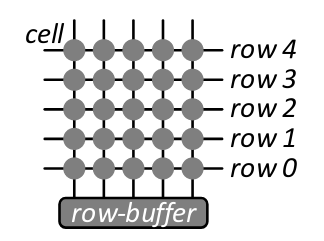
\includegraphics[width=0.6\textwidth]{images/cellrows.png}
    \caption*{\textbf{a.} Rows of Cells}
  \end{minipage}%
  \begin{minipage}{0.3\textwidth}
    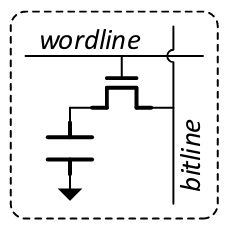
\includegraphics[width=0.6\textwidth]{images/singlecell.png}
    \caption*{\textbf{b.} Single Cell}
  \end{minipage}
  \caption{DRAM cell structure\cite{kimFlippingBitsMemory2014}}
\end{figure}

For instance, this code sequence
resulted in numerous bit flips, which varied across different
microarchitectures, as shown in Table \ref{tab:bit-flips} from the original paper:

  \begin{table}[htbp]
    \centering
    \label{tab:bit-flips}
    \begin{tabular}{lcccc}
    \toprule
    Bit-Flip     & Sandy Bridge & Ivy Bridge & Haswell & Piledriver \\
    \midrule
    `0` \textrightarrow\ `1` & 7,992       & 10,273     & 11,404   & 47         \\
    `1` \textrightarrow\ `0` & 8,125       & 10,449     & 11,467   & 12         \\
    \bottomrule
    \end{tabular}
    \caption{Bit-flips induced by disturbance on a 2GB module\cite{kimFlippingBitsMemory2014}}
    \label{tab:bit-flips}
  \end{table}

The ability to induce such bit flips remotely through crafted payloads 
has elevated Rowhammer from a
theoretical concern to a practical cybersecurity threat. The
implications of such a vulnerability are profound: systems could
potentially be compromised without the attacker ever physically touching
the hardware. This shifts the landscape of system security, emphasizing
the need for vigilant memory management and robust protective mechanisms
in both hardware design and system software.

\begin{enumerate}
  \def\labelenumi{\arabic{enumi}.}
  \setcounter{enumi}{3}
  \item
    \textbf{Modern Challenges}: Today, hardware vulnerabilities like
    \textbf{Spectre and Meltdown}\cite{SpectreSecurityVulnerability2024,MeltdownSecurityVulnerability2024} have shown that even fundamental
    hardware design principles can introduce security risks. These
    vulnerabilities exploit speculative execution---a performance feature in modern CPUs---to leak sensitive information. Speculative execution is used by CPUs to predict future execution paths and prematurely execute instructions without knowing if they are actually necessary\cite{lampsonLazySpeculativeExecution2006, raghavanDynamicSchemesSpeculative1998}. This can increase performance but also introduces the possibility of leaking information if the prediction is incorrect and the speculative execution has side effects that are not fully discarded.
  
    For instance, Spectre attacks trick the processor into executing instructions that should not have been executed, exploiting the latency in the branch prediction mechanism of the CPU. The processor's speculative execution feature is then leveraged to perform operations that leave observable side effects such as changes in cache state, even if the speculative results are discarded. These side effects can be monitored to infer sensitive data like cryptographic keys or personal information.\cite{kocherSpectreAttacksExploiting2018}
  
    \begin{minted}[frame=single, linenos, breaklines]{javascript}
    if (index < simpleByteArray.length) {
        index = simpleByteArray[index | 0];
        index = (((index * 4096)|0) & (2**25 - 1))|0;
        localJunk ^= probeTable[index|0]|0;
    }
    \end{minted}
    \label{lst:spectre}
    \captionof{lstlisting}{Speculative Execution Exploit via JavaScript.}

      In the paper, they present a straightforward JavaScript attack (Listing \ref{lst:spectre}) that, when run in a web browser, allows JavaScript code to read arbitrary memory locations, potentially leaking sensitive information.

      Alongside \textbf{Spectre}, the \textbf{Meltdown} vulnerability has revealed critical risks inherent in performance optimization techniques employed by modern CPUs. Specifically, Meltdown circumvents memory isolation guarantees by exploiting out-of-order execution, a feature used by CPUs to speed up processing. This exploitation allows an attacker to read all memory on a system, even without any permissions\cite{lippMeltdown2018}.

      Meltdown is based on a fundamental hardware behavior involving out-of-order execution, where CPUs execute instructions out of their planned sequence for efficiency. When the CPU processes an instruction that should not be executed, it discards the result to maintain correct program operation. However, the discarded results can affect the cache, leading to a potential side-channel that can be exploited.
      
      \begin{figure}[H]
        \centering
        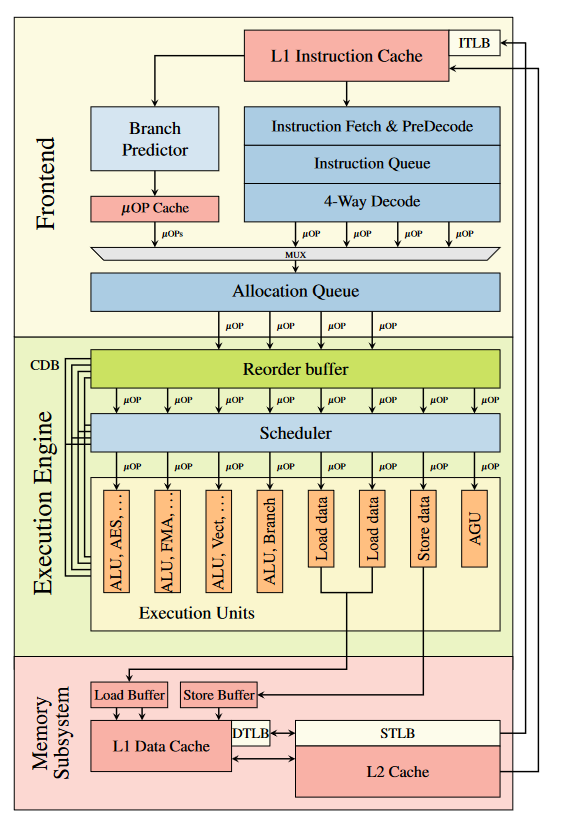
\includegraphics[width=0.6\textwidth]{images/intel-cpu.png}
        \caption{Simplified illustration of a single core of Intel's Skylake microarchitecture.\cite{lippMeltdown2018}}
        \label{fig:meltdown}
      \end{figure}
      
      Essentially, Meltdown breaks the foundational security boundary that segregates the kernel's memory space from user processes. Attackers can take advantage of Meltdown to access not just the kernel memory but the entire physical memory of the host machine, potentially exposing sensitive data across user processes and virtual machines. The issue is pervasive across numerous Intel CPUs and potentially other processors.
      
      \begin{minted}[frame=single, linenos, breaklines]{asm}
        ; rcx = kernel address 
        ; rbx = probe array 
        retry: 
          mov al, byte [rcx] 
          shl rax, 0xc 
          jz retry
          mov rbx, qword [rbx + rax]
      \end{minted}
      \captionof{lstlisting}{Meltdown Attack Assembly Code.}
      
      Unlike Spectre, Meltdown does not need to be tailored to a specific victim's environment, nor does it rely on any form of software vulnerability, making it widely exploitable on affected systems.     
\end{enumerate}
      
\hypertarget{milestones}{%
\subsection{Milestones}\label{milestones}}

\begin{itemize}
\item
  \textbf{1980s-1990s}: Radiation hardening techniques developed for
  space and military use.
\item
  \textbf{Early 2000s}: Rise of consumer electronics security with DRM
  and content protection.
\item
  \textbf{2014}: Discovery of the Rowhammer vulnerability, illustrating
  a shift towards remote exploitability of hardware.
\item
  \textbf{2018}: Spectre and Meltdown vulnerabilities exposed,
  highlighting deep-seated issues in CPU design.
\end{itemize}

Diving deeper into the Types of Hardware Flaws (cf.\ref{types-of-hardware-flaws}), we'll
explore the various categories of hardware vulnerabilities, providing a
more nuanced understanding of these threats through detailed examples,
code snippets, and references to academic and industry sources.

\hypertarget{types-of-hardware-flaws}{%
\section{Types of Hardware Flaws}\label{types-of-hardware-flaws}}

Hardware vulnerabilities can manifest in numerous forms, each exploiting
different aspects of physical design, implementation, and operational
behavior. These vulnerabilities are typically categorized into three
primary types: physical vulnerabilities, side-channel attacks, and fault
injection attacks.

\hypertarget{physical-vulnerabilities}{%
\subsection{Physical
Vulnerabilities}\label{physical-vulnerabilities}}

Physical vulnerabilities are those that necessitate direct interaction
with or access to the hardware device. They can exploit inherent design
flaws or result from malicious physical modifications.

\begin{itemize}
\item
  \textbf{Cold Boot Attacks}: A striking example of a physical
  vulnerability is the cold boot attack\cite{haldermanLestWeRemember2009}, 
  where sensitive data such as
  cryptographic keys are retrieved from RAM after a device is powered
  off. As described in the foundational paper, data remanence (residual physical representation of data that has been nominally erased or removed) in DRAM can persist for seconds to minutes at room
  temperature, and cooling the chips can extend this period
  significantly, allowing attackers to reboot the system with a custom
  loader and extract the remaining data.

  Post-cooling, an attacker uses a custom memory imaging tool to read the remaining data by rebooting the system with a minimal kernel that dumps the memory contents.
  The primary goal of that attack being the extraction of cryptographic keys from the decayed memory images, which are then used to decrypt sensitive data.

\item
  \textbf{Hardware Implantation}: Another form of physical vulnerability
  involves tampering with hardware components to introduce malicious
  functionality. For instance, adding a small, inconspicuous chip to a
  motherboard can create a backdoor for attackers to access or
  manipulate the device remotely.
  One prominent example of this is the \textbf{Stuxnet worm}, which targeted Iran's nuclear program by infecting the Programmable Logic Controllers (PLCs) used in uranium enrichment centrifuges. 
  Stuxnet exploited vulnerabilities in Windows systems to gain access to the PLCs, where it manipulated the centrifuge speeds to cause physical damage. 
  This attack demonstrated the potential for hardware implants to disrupt critical infrastructure and highlighted the need for robust hardware security measures.\cite{kushnerRealStoryStuxnet2013,nicolasfalliereW32StuxnetDossier}
\end{itemize}

\hypertarget{side-channel-attacks}{%
\subsection{Side-channel Attacks}\label{side-channel-attacks}}

Side-channel attacks exploit indirect effects of system operations, such
as timing, power consumption, and electromagnetic emissions, to infer
sensitive information without breaching the system's logical security
boundaries.

\subsubsection{Timing Attacks}

The seminal work of Kocher (1996)\cite{kocherTimingAttacksImplementations1996} on timing attacks offers a comprehensive examination of the vulnerabilities 
inherent in cryptographic systems due to variations in execution time during cryptographic operations such as modular exponentiation used in algorithms 
like RSA and Diffie-Hellman.

These attacks measure the time required for cryptographic operations,
using variations to deduce secret keys. For instance, by measuring the
time it takes for a server to respond to varying encrypted messages, an
attacker can infer details about the encryption keys.

Kocher models the timing attack as a signal detection problem, where the `signal' is the timing variation caused by the specific exponent bit, and `noise' consists of measurement inaccuracies and variations from unknown exponent bits. Extensive statistical analysis is utilized, focusing on the probability distribution function \( F \), which encapsulates the expected timing variations due to specific bits.

In practical scenarios, Kocher suggests simplifying the attack by avoiding the computation of \( F \). Instead, the focus shifts to analyzing the variance of timing measurements adjusted for each guessed exponent bit. If the guess is correct, the variance of these adjusted measurements will be lower than those adjusted for incorrect guesses.

This method of variance analysis serves as a crucial mechanism for efficiently distinguishing between correct and incorrect guesses of the secret key bits.

The paper includes experimental results using the RSA encryption algorithm implemented with the RSAREF toolkit, confirming that correct guesses about exponent bits consistently result in lower timing variances, thus validating the theoretical model. Kocher also discusses the potential for adapting the timing attack methodology to other cryptographic operations, underscoring its flexibility and broad applicability.\\

\begin{minted}[frame=single, linenos, breaklines]{python}
  def perform_timing_attack(modexp, n, base, public_exponent):
      timings = []
      guessed_exponent = 0
  
      for bit_position in range(number_of_bits(n)):
          best_time = float('inf')
          best_bit = None
  
          for bit in [0, 1]:
              test_exponent = set_bit(guessed_exponent, bit_position, bit)
  
              start_time = current_time()
              modexp(base, test_exponent, n)
              elapsed_time = current_time() - start_time

              if elapsed_time < best_time:
                  best_time = elapsed_time
                  best_bit = bit
  
          guessed_exponent = set_bit(guessed_exponent, bit_position, best_bit)
          timings.append((bit_position, best_time))
  
      return guessed_exponent, timings
  
  def number_of_bits(n):
      return n.bit_length()
  
  def set_bit(number, position, value):
      mask = 1 << position
      return (number & ~mask) | (value << position)
  
  def current_time():
      import time
      return time.time()
\end{minted}
\captionof{lstlisting}{Pseudocode for a timing attack}

\subsubsection{Power Analysis Attacks}

By monitoring the power usage of a device, attackers can gain insights into the data being processed. Simple Power Analysis (SPA) and Differential Power Analysis (DPA) are two common methods, with DPA being particularly effective at extracting cryptographic keys from seemingly innocuous power usage patterns.
We'll delve into how these attacks work by analyzing the work of Kocher et al. (1999)\cite{kocherDifferentialPowerAnalysis1999}.

\begin{itemize}
  \item \textbf{SPA}: In Single Power Analysis (SPA), we observe the power consumption of a device to infer the operations being executed. SPA can reveal significant information about the execution path of cryptographic algorithms.
  In SPA, the observable feature is the power consumption, which correlates with the physical operations of a device. 

  This type of analysis can detect significant operations within cryptographic algorithms, such as DES, by observing the distinct power signatures corresponding to each phase of the operation, notably the permutations and conditional operations based on the secret key.

  \begin{minted}[frame=single, linenos, breaklines]{python}
  def square_and_multiply(base, exponent, modulus):
    binary_exponent = bin(exponent)[2:]
    result = 1
    for bit in binary_exponent:
        result = (result * result) % modulus
        if bit == '1':
            result = (result * base) % modulus
    
    return result
  \end{minted}
  \captionof{lstlisting}{Pseudocode for a Single Power Analysis attack using `square and multiply' algorithm}
\end{itemize}

\begin{itemize}
  \item \textbf{DPA}: Differential Power Analysis uses statistical techniques to extract secret keys by analyzing power consumption data from multiple operations.
  In DPA, we focus on the mean difference of grouped data based on hypothetical intermediate values. Given a set of power traces \( T_i \) and a hypothesis function \( H(k, x) \) that predicts power consumption based on key guess \( k \) and input \( x \), the differential trace \( D \) is calculated as:
\[
D_k[j] = \frac{1}{|G_0|} \sum_{i \in G_0} T_i[j] - \frac{1}{|G_1|} \sum_{i \in G_1} T_i[j]
\]
where \( G_0 \) and \( G_1 \) are sets of indices classified by whether \( H(k, x_i) \) predicts low or high power consumption, respectively.

\begin{minted}[frame=single, linenos, breaklines]{python}
  def dpa_attack(traces, key_guesses):
    high_group = []
    low_group = []
    for trace, key_guess in zip(traces, key_guesses):
        if predict_high(key_guess):
            high_group.append(trace)
        else:
            low_group.append(trace)
    mean_high = np.mean(high_group, axis=0)
    mean_low = np.mean(low_group, axis=0)
    return mean_high - mean_low
\end{minted}
\captionof{lstlisting}{Pseudocode for a Differential Power Analysis attack}

In this pseudocode, \texttt{traces} is a list of power consumption traces, and \texttt{key\_guesses} is a list of key hypotheses. The function \texttt{predict\_high} decides the grouping based on a prediction model using the key guess. The differential trace, computed as the difference between the means of these groups, helps identify the correct key guess by highlighting variations in the power consumption corresponding to different key bits.

\end{itemize}

\subsubsection{Fault Injection Attacks}

Fault injection attacks deliberately induce operational errors to bypass security mechanisms or corrupt the execution of processes, exploiting these faults for unauthorized access or data extraction.

\begin{itemize}
\item \textbf{Voltage Glitching}: A technique used to manipulate the physical operating conditions of electronic devices in order to induce faults. These faults can be exploited to bypass security measures or corrupt the device's usual execution flow. In the context of security research, voltage glitching is often applied to cryptographic devices to either bypass security checks or extract secret keys.

The basic idea behind voltage glitching involves momentarily altering the device's power supply to disrupt its normal operation. This disruption can cause the device to skip instructions, execute incorrect instructions, or produce erroneous data.\cite{bar-elSorcererApprenticeGuide2004}

In practical scenarios, such as the one explored by Moradi et al.\cite{moradiVulnerabilityFPGABitstream2011} in their research on FPGA bitstream encryption vulnerabilities, voltage glitching is used to manipulate the execution of cryptographic algorithms, allowing attackers to bypass security checks or interfere with the encryption process.\\

\begin{minted}[frame=single, linenos, breaklines]{python}
def voltage_glitching_attack(target_operation):
  successful = False
  while not successful:
    apply_voltage_drop()
    result = target_operation()
    
    if check_for_errors(result):
      exploit_errors(result)

    successful = True
\end{minted}

Voltage glitching poses significant security risks, particularly for devices that handle sensitive information like cryptographic keys.

As discussed by Bittner et al. (2021)\cite{bittnerForgottenThreatVoltage2021}, voltage glitching remains a potent attack vector against electronic devices, especially as hardware becomes increasingly miniaturized and integrated.

\begin{figure}[H]
  \centering
  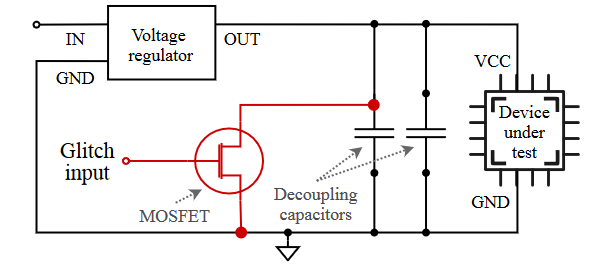
\includegraphics[width=0.6\textwidth]{images/glitch.png}
  \caption{Voltage glitching attack on a microcontroller\cite{bittnerForgottenThreatVoltage2021}}
  \label{fig:voltage_glitching}
\end{figure}

Voltage glitching has been adapted to target advanced microarchitectures and security-enforced environments. Modern devices often incorporate complex power management features that can be exploited to introduce glitches more subtly and effectively
\end{itemize}

\begin{itemize}
\item
  \textbf{Clock Glitching}: Similar to voltage glitching, clock
  glitching involves momentarily altering the system clock's frequency or timing, disrupting the sequence of
operations and potentially allowing attackers to manipulate or bypass
processes.\cite{bar-elSorcererApprenticeGuide2004}

It exploits vulnerabilities in the timing mechanisms of digital circuits, like those identified in that research\cite{tajikPhysicalCharacterizationArbiter2014}. This study demonstrates that high-resolution photonic emission analysis can physically characterize the intrinsic behavior of timing-based security mechanisms, such as those found in arbiter Physical Unclonable Functions (PUFs), by measuring the minute delays within the circuit with great precision. The relevance of this technique to clock glitching lies in its ability to manipulate and observe the effects of slight deviations in clock frequency or pulse timing, which can induce errors or alter the behavior of the security mechanism. This method provides a potent example of how even robust security designs can be undermined by exploiting their fundamental physical properties—highlighting a critical area for enhancing resistance to clock glitching attacks

\begin{minted}[frame=single, linenos, breaklines]{python}
  def clock_glitching_attack(target_device):
      original_clock = target_device.clock
      while not achieved_goal:
          glitched_clock = induce_clock_glitch(original_clock)
          target_device.clock = glitched_clock
          if target_device.malfunctions():
              exploit_malfunction(target_device)
          target_device.clock = original_clock 
  \end{minted}
  \captionof{lstlisting}{Pseudocode for a clock glitching attack}

\end{itemize}

\hypertarget{mitigation-strategies}{%
\section{Mitigation Strategies}\label{mitigation-strategies}}

Mitigation strategies in hardware security encompass a wide array of
techniques, from design-phase interventions to post-incident responses.
These strategies are essential for reducing the risk and impact of
hardware vulnerabilities.

\hypertarget{preemptive-measures}{%
\subsection{Preemptive Measures}\label{preemptive-measures}}

\textbf{Secure Hardware Design}: Embedding security features at the
design level can significantly reduce vulnerabilities. This includes the
adoption of design practices that inherently minimize security risks,
such as:

\begin{itemize}
\item
  \textbf{Redundant Design}: Implementing redundant circuits to provide
  fallback options in case of failure or tampering.

  \begin{minted}[frame=single, linenos, breaklines]{python}
    def execute_secure_operation(operation, redundancy_level=2):
        results = []
        for _ in range(redundancy_level):
            result = operation()
            results.append(result)
        if all_equal(results):
            return results[0] 
        else:
            raise SecurityException("Discrepancy detected in redundant operations")
    \end{minted}
    \captionof{lstlisting}{Pseudocode for redundant design implementation}
    
\item
  \textbf{PUFs}: Utilizing unique
  physical characteristics of the hardware as cryptographic keys or
  identifiers, enhancing security against cloning and tampering.

  In their exploration of RO-PUFs\cite{maitiLargeScaleCharacterization2010}, Maiti detailed the deployment of ring oscillator PUFs on a large array of FPGA chips to analyze the viability of PUFs in achieving high levels of hardware security through uniqueness and reliability. RO-PUFs utilize the minute variations in the oscillation frequency of identically laid-out ring oscillators, which arise due to unavoidable process variations during chip manufacturing. These frequencies are sensitive to environmental conditions and operational variations, which in turn, affect the reliability of the PUF's response.

  The uniqueness of a PUF is measured by the inter-die Hamming distance, which should ideally be close to 50\%. Maiti demonstrated that RO-PUFs achieve an average inter-die Hamming distance of 47.31\%, which indicates a high level of uniqueness in responses across different chips.l
\end{itemize}

\textbf{Hardware-assisted Security}: Modern processors have integrated features to bolster security at the hardware level, notably Intel's Software Guard Extensions (SGX)\cite{costanIntelSGXExplained2016} and AMD's Secure Encrypted Virtualization (SEV)\cite{mofradComparisonStudyIntel2018}. These technologies enhance the protection of sensitive code and data within secure enclaves or encrypted virtual machines, shielding them from potentially compromised privileged software.

\begin{itemize}
\item
  \textbf{Intel SGX}: Intel's Software Guard Extensions (SGX) provide a way to increase the security of software systems on platforms where the privileged software, like the operating system or hypervisor, might be compromised. SGX achieves this by allowing sensitive computations to take place within a protected area of execution, called an enclave, which is designed to be tamper-resistant even from privileged code running on the same machine.

  based on the paper by Costan and Devadas\cite{costanIntelSGXExplained2016}, SGX designates a region of memory known as Processor Reserved Memory (PRM), where the sensitive code and data reside. This region is protected by the CPU such that no non-enclave memory access can occur, including those from the kernel, hypervisor, System Management Mode (SMM), and Direct Memory Access (DMA) from peripherals.

  Within PRM, there's a structure called the Enclave Page Cache (EPC), consisting of 4 KB pages that store the actual code and data of enclaves. System software, which is not fully trusted, is responsible for assigning these pages to enclaves, but the CPU ensures through the Enclave Page Cache Metadata (EPCM) that each page is only associated with a single enclave.

  The SGX framework aims to enable secure remote computation by allowing users to run security-sensitive applications on a remote computer, potentially operated by an untrusted party, with integrity and confidentiality guarantees. Users can safely upload encrypted data and code for processing in a secure enclave, with the knowledge that the enclave is protected against tampering or unauthorized access, even from the host system's privileged software.

\item
  \textbf{AMD SEV}: AMD's Secure Encrypted Virtualization (SEV) is a hardware feature designed to encrypt the memory of virtual machines (VMs), aiming to protect the memory contents against unauthorized access, even from privileged software like hypervisors.

  From the paper by Mofrad et al.\cite{mofradComparisonStudyIntel2018}, SEV is built upon AMD's Memory Encryption Technology, which employs a dedicated AES engine within the system on a chip (SoC) to encrypt and decrypt memory pages on the fly, without noticeable performance impact to the user.

  Each VM under SEV has its own unique encryption key, which is managed by the AMD Secure Processor, an ARM Cortex-A5 core within the SoC. This ensures that even if one VM’s security is compromised, the others remain protected due to the use of separate keys.

  SEV aims to protect against both direct memory attacks (such as cold-boot attacks) and indirect attacks that exploit the hypervisor (such as side-channel attacks).

  Unlike Intel SGX, which provides memory integrity protection, AMD SEV does not protect the integrity of the encrypted VM memory. However, the use of AMD's secure processor to manage encryption keys keeps these keys out of the reach of the hypervisor or any other privileged code on the host.

  While SEV provides robust protection against many types of attacks, it does not completely eliminate the risk of security breaches. For example, side-channel attacks and other sophisticated exploits remain a concern.

  AMD has responded to security vulnerabilities with firmware updates, indicating that while SEV provides a significant security advantage, it requires ongoing maintenance and updates to ensure the highest level of protection.
\end{itemize}

\textbf{Side-channel Resistance}: Side-channel resistance is crucial in cryptographic implementations to prevent leakage of sensitive information through unintended channels. Techniques such as constant-time programming and differential power analysis (DPA) resistance are pivotal to enhancing the security of cryptographic systems.

The primary defense against timing attacks is ensuring that operations execute in constant time. Timing attacks exploit the variable execution times of operations depending on secret values. Just like the OpenSSL `memcmp' function\cite{DocsMan1Man3}.\\

\begin{minted}[frame=single, linenos, breaklines]{c}
  int constant_time_memcmp(const void* a, const void* b, size_t size) {
      const unsigned char* _a = (const unsigned char*)a;
      const unsigned char* _b = (const unsigned char*)b;
      unsigned char result = 0;
      for (size_t i = 0; i < size; i++) {
          result |= _a[i] ^ _b[i];
      }
      return result == 0;
  }
  \end{minted}  
  \captionof{lstlisting}{Simplified constant-time comparison function in C for understanding.}

  DPA attacks involve analyzing power consumption patterns during cryptographic operations to infer secret keys. Countermeasures include balancing power consumption across different operations and using randomization techniques to mask the power signature. Cryptographic algorithms can be modified to exhibit uniform power consumption, or additional circuitry can be integrated to disguise the actual power use patterns.

  Modern cryptographic modules integrate side-channel resistant features, including noise generators and dual-rail logic, to obscure the relationship between the cryptographic operations and the physical emissions like power or electromagnetic signals.

  Dedicated hardware elements, such as Hardware Security Modules (HSMs) or Trusted Platform Modules (TPMs), often include designs that inherently resist side-channel attacks, thereby safeguarding the cryptographic processes they handle.
  
\hypertarget{reactive-strategies}{%
\subsection{Reactive Strategies}\label{reactive-strategies}}

\textbf{Firmware and Software Updates}: Patching vulnerabilities is a
common approach to mitigate discovered flaws. This includes updates to:

\begin{itemize}
\item
  \textbf{Microcode} is a layer of low-level code that governs the behavior of the processor's hardware. It plays a crucial role in the functionality of CPUs by interpreting high-level machine instructions into sequences of low-level operations specific to the processor. When vulnerabilities are discovered within this layer, microcode updates are issued to mitigate these issues.\cite{kentEncyclopediaComputerScience1993}

  One notable example of microcode being used to address a significant vulnerability is in the mitigation of the Spectre and Meltdown vulnerabilities. These vulnerabilities exploit critical flaws in modern processors, allowing malicious programs to steal data being processed on the computer. Manufacturers like Intel released microcode updates to reduce the risk of these vulnerabilities, although sometimes at the cost of degraded system performance \cite{burkeIntelUnleashesComprehensive}
\item
  \textbf{Device Firmware} refers to the fixed, often proprietary software that provides the necessary instructions for how a device operates. This can include everything from the basic operating system of an embedded device, like a network router or a smart thermostat, to the BIOS/UEFI firmware of a personal computer.\cite{WhatFirmware2013}

  Updating device firmware can enhance the security of peripherals and embedded systems by patching vulnerabilities as they are discovered. A well-known case involved the exploitation of vulnerabilities in the firmware of wireless routers. Manufacturers regularly release firmware updates to patch these security holes and add new features or improvements.

\end{itemize}

\textbf{Hardware Recalls and Replacements}: In cases where software
cannot fully mitigate a vulnerability, hardware modifications or recalls
may be necessary.

\begin{itemize}
\item
  \textbf{TPM Recalls}: The Trusted Platform Module (TPM) is designed to secure hardware through integrated cryptographic keys. When a vulnerability was discovered in Infineon TPMs, it was found that the RSA keys generated by these modules were not as secure as expected, making them susceptible to cryptographic attacks. This led to a recall and hardware fix to replace the vulnerable TPMs, highlighting a scenario where firmware updates alone were insufficient to secure the hardware.cite{InfineonRSAKey2021}
\end{itemize}

\textbf{Isolation and Virtualization}: Employing hardware and software
techniques to isolate potentially vulnerable components or sensitive
operations from the rest of the system.

\begin{itemize}
\item
  \textbf{Virtualization-Based Security (VBS)}: Uses hardware
  Virtualization-Based Security (VBS) leverages hardware virtualization features to create isolated secure regions of memory away from the normal operating system. This can protect sensitive data and operations even if the operating system is compromised. An example of VBS in action is Microsoft's use of it in Windows Defender Credential Guard, which isolates secrets so that only privileged system software can access them, thus protecting against pass-the-hash or pass-the-ticket types of attacks.\cite{vinaypamnani-msftWindowsDefenderApplication2024}
\end{itemize}

\hypertarget{current-challenges-in-hardware-security}{%
\section{Current Challenges in Hardware
Security}\label{current-challenges-in-hardware-security}}

\hypertarget{complexity-and-integration}{%
\paragraph{Complexity and
Integration}\label{complexity-and-integration}}

Every day, hardware devices become more integrated and complicated, expanding the potential for security flaws. Today's hardware, like System on Chips (SoCs) in smartphones or IoT devices, integrates numerous functionalities such as processors, memory, and connectivity options into single chips. This high level of integration raises the risk of cross-component vulnerabilities.

Spectre and Meltdown vulnerabilities are a good exemple of this, that exploit critical issues in modern processors. These vulnerabilities essentially leverage the complexity of speculative execution—a feature designed to enhance CPU performance—to allow an attacker to access sensitive data. The risk was amplified because these processors are used across a wide array of devices, illustrating how integration and complexity can expose multiple systems to a single point of failure.\cite{kocherSpectreAttacksExploiting2018}

\hypertarget{scaling-of-preemptive-measures}{%
\paragraph{Scaling of Preemptive
Measures}\label{scaling-of-preemptive-measures}}

As hardware technologies evolve, scaling preemptive security measures becomes a formidable challenge. Each new generation of hardware not only needs to incorporate defenses against known threats but must also be designed with the foresight to handle emerging vulnerabilities. This involves a delicate balance of performance, security, and power consumption considerations.

For instance, Trusted Execution Environments (TEEs) like ARM's TrustZone are designed to offer a secure area of the main processor to run sensitive code in isolation from the main operating system. As hardware evolves, these environments need continuous updates to mitigate new kinds of attacks, which might include sophisticated malware that can breach isolated environments.\cite{ngabonzizaTrustZoneExplainedArchitectural2016}

\hypertarget{post-quantum-cryptography}{%
\paragraph{Post-Quantum Cryptography}\label{post-quantum-cryptography}}

The emergence of quantum computing presents a potential threat to current cryptographic standards, which could undermine the security of communications and data protection. This drives the need for post-quantum cryptography (PQC), which involves developing cryptographic systems that are secure against both quantum and classical computers and can be integrated into existing communications protocols and hardware.

The National Institute of Standards and Technology (NIST) has been actively working on standardizing post-quantum cryptographic algorithms. This effort is critical as it anticipates the quantum threat to ensure the long-term security of public key encryption, digital signatures, and key establishment protocols in hardware.\cite{computersecuritydivisionPostQuantumCryptographyCSRC2017}

\hypertarget{reactive-strategy-limitations}{%
\paragraph{Reactive Strategy
Limitations}\label{reactive-strategy-limitations}}

Hardware's inherent inflexibility makes it challenging to address vulnerabilities through reactive measures post-production. Unlike software, which can often be patched with updates, hardware may require physical replacements or recalls if a critical vulnerability is discovered. This approach is not only costly but also logistically challenging.

A notable case is the Infineon TPM recall, like we talked about before, where the hardware-based security tool had to be physically replaced due to vulnerabilities in key generation. This situation underscores the high stakes and costs involved in reactive strategies for managing hardware security vulnerabilities.

\hypertarget{future-research-directions}{%
\subsection{Future Research
Directions}\label{future-research-directions}}

\hypertarget{advanced-materials-and-fabrication-techniques}{%
\paragraph{Advanced Materials and Fabrication
Techniques}\label{advanced-materials-and-fabrication-techniques}}

Exploring advanced materials and new fabrication techniques offers promising avenues for enhancing hardware security. Materials like graphene, known for its exceptional strength and electrical conductivity, could potentially be used to develop hardware that is inherently resistant to tampering and offers improved electromagnetic shielding.

Research in nanoscale fabrication techniques might also enable the creation of hardware components that are smaller, faster, and more energy-efficient, while also being more difficult to physically tamper with or reverse engineer. For example, using three-dimensional integrated circuits (3D ICs) can enhance device performance and security by vertically stacking and interconnecting multiple layers of components.\cite{GrapheneStrongLightweight, kavandSecuringHardwareReconfigurable2022}

\hypertarget{ai-and-machine-learning-for-security}{%
\paragraph{AI and Machine Learning for
Security}\label{ai-and-machine-learning-for-security}}

Integrating artificial intelligence (AI) and machine learning (ML) directly into hardware can provide dynamic and adaptive security measures. AI-driven systems could be designed to detect and respond to security breaches in real-time by learning from ongoing attacks and adapting to prevent similar vulnerabilities in the future.

Google's Titan M security chip, for instance, incorporates machine learning to detect patterns indicative of external tampering attempts. This chip secures the bootloader and critical security parameters at the hardware level, illustrating how integrating AI can enhance the security of hardware devices against sophisticated threats.

\hypertarget{homomorphic-encryption-hardware}{%
\paragraph{Homomorphic Encryption
Hardware}\label{homomorphic-encryption-hardware}}

Homomorphic encryption allows computations to be carried out on encrypted data, returning an encrypted result that, when decrypted, matches the result of operations performed on the plaintext. Developing specialized hardware that supports homomorphic encryption operations natively can revolutionize data privacy by enabling secure computation on encrypted data without ever needing decryption.

This technology is particularly crucial for cloud computing, where sensitive data can be processed without exposing it to cloud providers or other potential vulnerabilities. Research into efficient, scalable hardware solutions for homomorphic encryption is essential for the practical deployment of privacy-preserving computation in real-world applications.\cite{gentryFULLYHOMOMORPHICENCRYPTION}

\hypertarget{secure-hardware-lifecycle-management}{%
\paragraph{Secure Hardware Lifecycle
Management}\label{secure-hardware-lifecycle-management}}

The entire lifecycle of hardware, from design and manufacturing through to decommissioning, needs to be secured to prevent any potential security breaches. This includes secure supply chain practices, reliable firmware updates, and methods for safely decommissioning and recycling hardware without risking data leakage.

An example of a comprehensive approach to this is Secure Device Lifecycle Management (SDLM), which encompasses secure provisioning, ongoing maintenance updates, and secure end-of-life processes. Ensuring that hardware remains secure throughout its operational lifetime and beyond is vital to preventing long-term vulnerabilities.

\hypertarget{conclusion}{%
\section{Conclusion: Navigating the Landscape of Hardware Security}\label{conclusion}}

Hardware security is an increasingly critical domain within the broader field of cybersecurity, underscored by the myriad vulnerabilities, sophisticated attack vectors, and the dynamic nature of threats that modern computing systems face. From physical vulnerabilities like cold boot attacks to advanced exploitation techniques such as side-channel attacks and fault injection, the diversity and sophistication of threats necessitate a robust and multifaceted response.

Mitigating hardware vulnerabilities requires a strategic blend of preemptive and reactive measures. Preemptive strategies involve secure hardware design from the ground up, incorporating hardware-assisted security features, and robust cryptographic implementations to ward off potential threats. Reactive measures, although challenging due to the inherent rigidity of hardware, play a critical role in addressing vulnerabilities that surface after hardware deployment. These may include firmware updates, hardware modifications, or even recalls and replacements in cases where software solutions are insufficient.

The ongoing discovery of critical vulnerabilities, such as Rowhammer, Spectre, and Meltdown, highlights the continuous need for vigilance and innovation in the field of hardware security. These vulnerabilities have not only shown the potential for widespread impact across multiple platforms but also the necessity for a proactive approach in hardware security practices.

As technology evolves, so too does the complexity of the hardware that powers it. This progression demands that future research and development in hardware security not only keep pace with current technological advances but also anticipate future challenges. Innovations such as the integration of advanced materials, the application of AI and machine learning in security mechanisms, development of homomorphic encryption hardware, and comprehensive secure hardware lifecycle management are essential.

Ultimately, ensuring the security of hardware is fundamental to protecting the integrity and confidentiality of entire computing systems. It supports the safe execution of applications and the protection of data, serving as the cornerstone of trust and reliability in technology. As we look to the future, the field of hardware security must continue to evolve, adapting to new threats and leveraging innovative technologies to safeguard against both known and unknown vulnerabilities. This ongoing commitment to enhancing hardware security is crucial for maintaining the confidence and trust of users and industries that depend on these technologies.

\chapter{The Nintendo Switch and the Fusee Gelee Exploit}
\epigraph{quote}{\textit{author}}

\section{Nintendo Switch Security Overview}

\subsection{Security Architecture of the Nintendo Switch}

The Nintendo Switch, a popular gaming console, employs a multi-layered security architecture designed to protect both the hardware and software from unauthorized access and tampering. Central to this architecture is the use of a secure boot process, which ensures that only authenticated firmware and software can be executed on the device.

\subsection{The Role of Boot ROM and Secure Boot Process}

he Boot ROM is an essential component of the Switch's security architecture. It contains the initial code that is executed when the console is powered on. This code performs the critical task of verifying the integrity and authenticity of the subsequent stages of the boot process through cryptographic checks. The secure boot process involves several steps:

\begin{itemize}
    \item \textbf{ROM Code Execution}: The immutable Boot ROM code is executed first. This code is hardwired into the chip and cannot be modified post-manufacturing.
    \item \textbf{Verification of Bootloader}: The Boot ROM verifies the digital signature of the bootloader stored in non-volatile memory.
    \item \textbf{Loading and Executing Bootloader}: Upon successful verification, the bootloader is loaded into memory and executed, which in turn verifies and loads the operating system kernel.
\end{itemize}

This chain of trust is designed to prevent unauthorized code from running on the device, thereby protecting the system from low-level attacks.

\section{Discovery of Fusee Gelee Exploit}

\subsection{Technical Specifics of the Vulnerability}

The Fusee Gelee exploit, discovered by the hacking team ReSwitched, leverages a critical vulnerability in the Nvidia Tegra X1 chip used in the Nintendo Switch. The exploit targets a flaw in the USB recovery mode of the Tegra chip. Specifically, the vulnerability arises from an unchecked buffer during the handling of USB control transfers in the Boot ROM code.

When a device enters USB recovery mode, it expects a specific sequence of USB packets. The vulnerability is triggered by sending an oversized control transfer, which overflows a buffer in the Boot ROM, allowing the attacker to execute arbitrary code. This type of vulnerability is known as a buffer overflow attack.

\subsection{Exploitation Mechanism}

The exploitation process involves several steps:

\begin{itemize}
    \item \textbf{Initiating Recovery Mode}: The attacker forces the Switch into USB recovery mode by shorting specific pins on the right Joy-Con connector, which triggers the device to await USB communication.
    \item \textbf{Sending Malicious USB Payload}: A specially crafted USB payload is sent to the device. This payload is designed to overflow the buffer and overwrite critical memory regions.
    \item \textbf{Executing Arbitrary Code}: The overwritten memory regions include the instruction pointer, which is redirected to execute the attacker’s payload. This payload typically includes a custom bootloader or code to bypass security checks.
\end{itemize} 

The execution of arbitrary code at such an early stage of the boot process effectively allows the attacker full control over the device, bypassing all subsequent security measures.

\section{Implications of the Exploit}

\subsection{Broader Implications within Hardware Security}

The Fusee Gelee exploit has significant implications for hardware security, highlighting several key challenges.

First, \textbf{inherent vulnerabilities in hardware} present a significant challenge because, unlike software, these flaws cannot be easily patched after the manufacturing process. The discovery of a critical vulnerability in a component like the Boot ROM highlights the necessity for rigorous security testing during the hardware design phase. Addressing hardware vulnerabilities is particularly difficult; once identified, remediation often requires physical modifications to the device or complete hardware revisions. Software patches alone are inadequate since they cannot alter the immutable Boot ROM code. The impact of such vulnerabilities is far-reaching, as illustrated by the Fusee Gelee exploit, which affects not only the Nintendo Switch but also other devices utilizing the same Tegra X1 chip. This example demonstrates how a single hardware flaw can have extensive consequences across various products and industries.

\subsection{Challenges in Addressing Embedded Hardware Vulnerabilities}

Addressing embedded hardware vulnerabilities involves several significant challenges. Detection and disclosure of such vulnerabilities require specialized knowledge and tools. It is crucial to follow responsible disclosure practices to prevent malicious exploitation while allowing manufacturers the necessary time to develop countermeasures. Implementing fixes for already deployed devices is both complex and costly. Hardware manufacturers must balance the need for security with the practicalities of providing hardware revisions or replacements to users. Future hardware designs must incorporate security from the ground up, utilizing principles like secure enclaves and hardware-based roots of trust to minimize the risk of similar vulnerabilities. The Fusee Gelee exploit serves as a stark reminder of the importance of proactive security measures in hardware design and the ongoing vigilance required to protect against evolving threats.
\chapter{Practical Analysis of the Fusee Gelee Exploit}
\epigraph{quote}{\textit{author}}
\chapter{Nintendo's Response and Industry Implications}
\epigraph{quote}{\textit{author}}
\chapter{Alternative Mitigation Strategies}
\epigraph{There's no silver bullet solution with cybersecurity; a layered defense is the only viable defense.}{\textit{James Scott}}

Nintendo's response to the Fusee Gelee exploit, involving both hardware revisions and software updates, has been largely effective in mitigating the immediate vulnerability. The introduction of the Mariko chip with a corrected Boot ROM and the release of new hardware models have addressed the specific buffer overflow issue exploited by Fusee Gelee. However, these measures have limitations, particularly in terms of financial accessibility for users and the residual vulnerability of older Switch models. Additionally, even the new consoles, while more secure, remain susceptible to hacking through more complex methods requiring advanced tools and techniques

\section{Proposed Solutions}
To further enhance the security of hardware like the Nintendo Switch, additional strategies beyond those implemented by Nintendo could be considered. These strategies aim to provide more comprehensive protection but come with their own set of drawbacks.

\subsection{Hardware-Level Solutions}
\subsubsection{Secure Enclave Integration}

One effective method for enhancing hardware security is the integration of secure enclaves. Secure enclaves are isolated execution environments within the processor that perform sensitive operations, such as cryptographic key storage and execution of critical code, in a protected manner.\cite{IntroductionHardwareSecurity}

\begin{figure}[H]
    \centering
    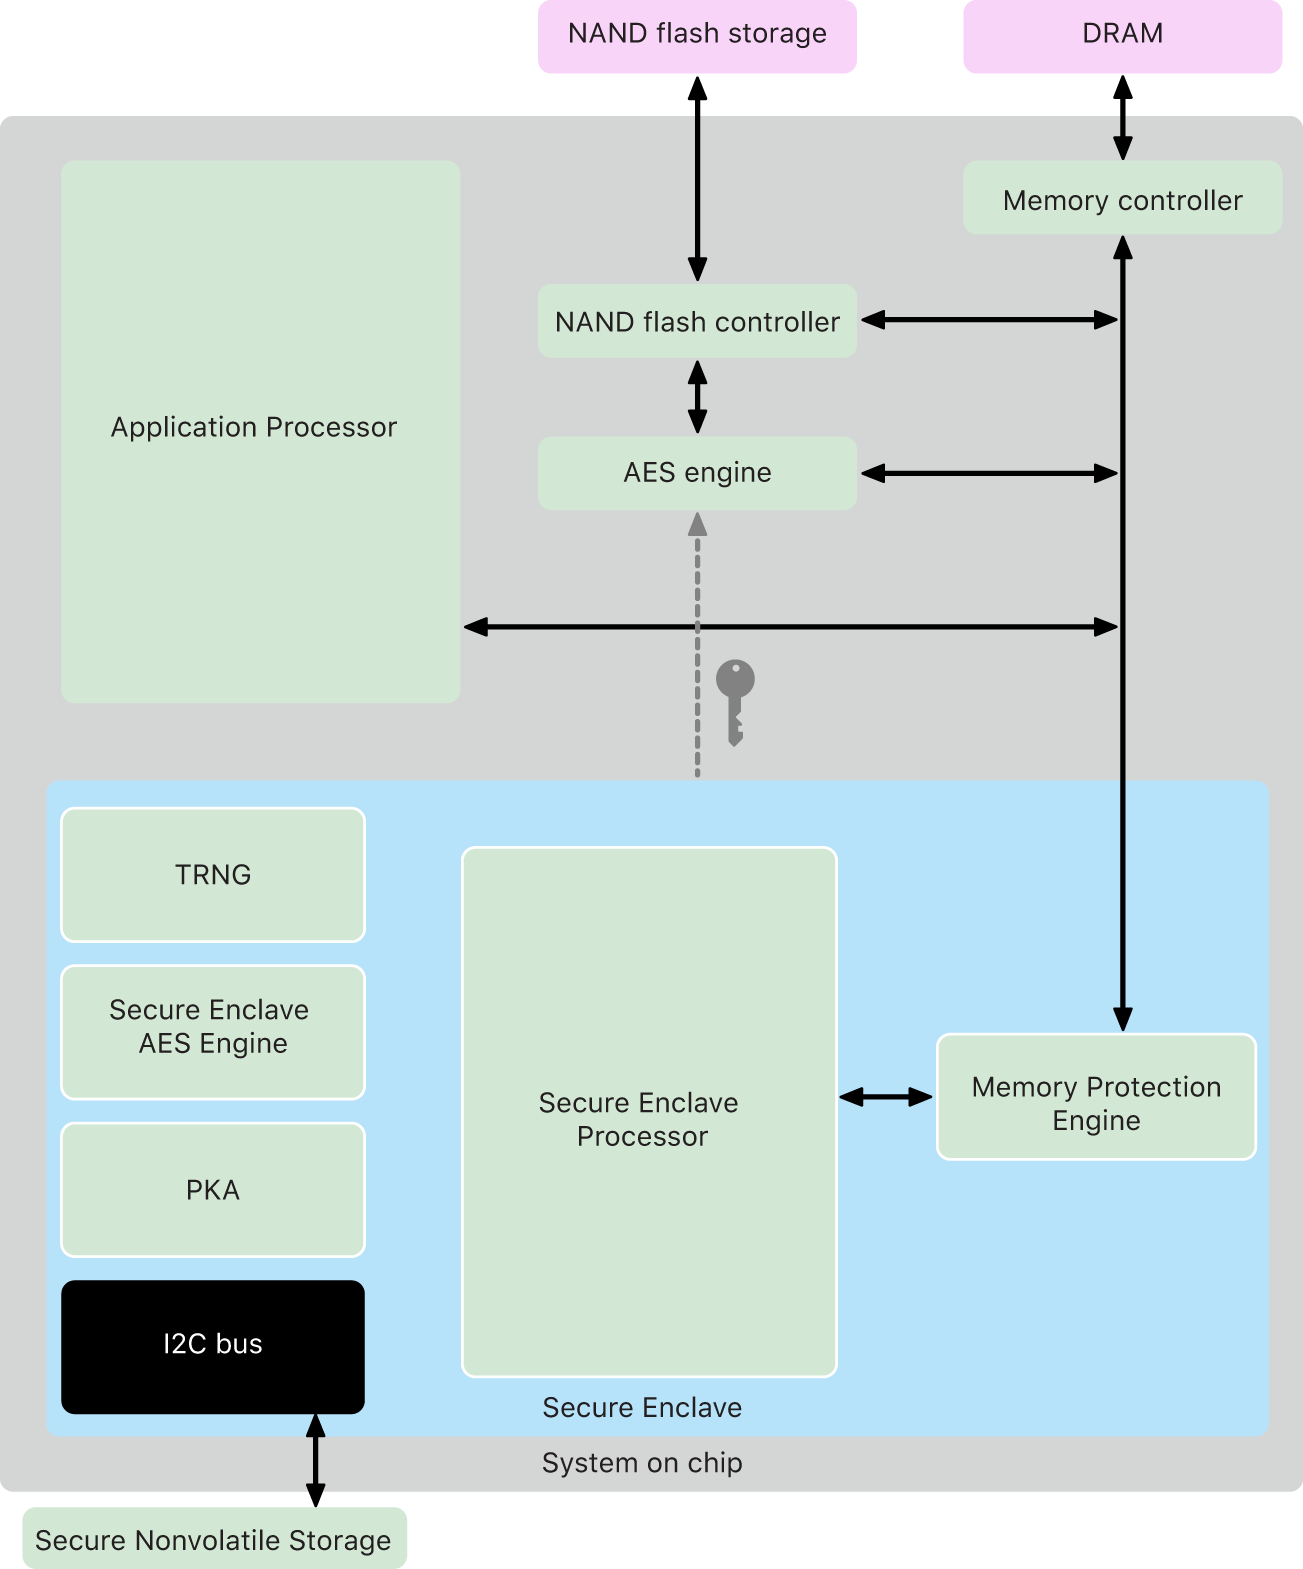
\includegraphics[width=.8\linewidth]{images/enclave.png}
    \caption{Secure Enclave Architecture from\cite{SecureEnclave}}
    \label{fig:secure_enclave}
\end{figure}

\subsubsection{Advantages}

\begin{itemize}
    \item \textbf{Enhanced Security}: Secure enclaves provide robust protection against a wide range of attacks, including those targeting the Boot ROM and other critical components.
    \item \textbf{Root of Trust}: They establish a hardware-based root of trust, ensuring that even if other parts of the hardware are compromised, sensitive operations remain secure.
\end{itemize}
\subsubsection{Drawbacks}

\begin{itemize}
    \item \textbf{Increased Cost}: Integrating secure enclaves into the hardware design significantly increases manufacturing costs.
    \item \textbf{Complexity}: It adds complexity to the hardware design and development process, potentially leading to longer development cycles and higher production costs
\end{itemize}
\subsubsection{Redundant Security Mechanisms}
Incorporating redundant security mechanisms\cite{RedundancyEngineering2023} can provide multiple layers of defense against hardware vulnerabilities. For example, dual verification processes during the boot sequence, where both the Boot ROM and a secondary chip verify each other's integrity, can enhance security.

\subsubsection{Advantages}

\textbf{Increased Reliability}: Multiple layers of verification reduce the likelihood of successful exploitation.
\textbf{Fault Tolerance}: Redundant systems provide a fallback in case one security measure is compromised.
\subsubsection{Drawbacks}

\begin{itemize}
    \item \textbf{Design Complexity}: Implementing redundant mechanisms increases the complexity of the hardware design.
    \item \textbf{Cost and Power Consumption}: Additional components and verification processes can increase both the cost and power consumption of the device.
\end{itemize}


\begin{figure}[H]
    \centering
    \begin{tikzpicture}[
        box/.style={rectangle, draw, text width=8em, align=center, rounded corners},
        arrow/.style={-Stealth, thick},
        level distance=2cm
      ]
      
      % Nodes
      \node[box] (bootrom) {Boot ROM Initiates Boot};
      \node[box, below=of bootrom] (verify1) {Verifies Secondary Chip Integrity};
      \node[box, below=of verify1] (secondary) {Secondary Chip Firmware};
      \node[box, right=of verify1, xshift=2cm] (verify2) {Verifies Boot ROM Integrity};
      
      % Paths
      \draw[arrow] (bootrom) -- (verify1);
      \draw[arrow] (verify1) -- (secondary);
      \draw[arrow] (secondary) -- ++(1.5cm, 0) |- (verify2);
      \draw[arrow] (verify2) -- ++(-1.5cm, 0) |- (verify1);
    \end{tikzpicture}
    \caption{Redundant Security Mechanisms in Boot Sequence}
    \label{fig:redundant_security}
\end{figure}

In conclusion, while Nintendo's response to the Fusee Gelee exploit has been effective to a large extent, further enhancements could be made by adopting advanced hardware. These measures, however, come with significant drawbacks, highlighting the inherent challenges in achieving complete security in consumer hardware devices. Future hardware designs must balance these trade-offs to ensure robust security while maintaining cost-effectiveness and performance.
\chapter{Conclusion}
\epigraph{Arguing that you don't care about the right to privacy because you have nothing to hide is no different than saying you don't care about free speech because you have nothing to say.}{\textit{Edward Snowden}}

\section{Summary of Findings}

This paper has explored the Fusee Gelee exploit in the Nintendo Switch, a significant hardware vulnerability that underscores the critical importance of hardware security. The study began with an overview of the Switch's security architecture, detailing the role of the Boot ROM and the secure boot process. It then examined the discovery and technical specifics of the Fusee Gelee exploit, which leverages an unchecked buffer in the Nvidia Tegra X1 chip's USB recovery mode to execute arbitrary code.

Through practical experimentation, the study validated the exploit's capability to bypass the secure boot process, allowing for arbitrary code execution. This finding highlights the fundamental vulnerability within the Tegra X1 chip's Boot ROM and demonstrates the severe implications of such hardware flaws.

\section{Contribution to Security}

The Fusee Gelee exploit serves as a critical case study in the field of hardware security, illustrating several key points:

\begin{itemize}
    \item \textbf{Inherent Vulnerabilities in Hardware}: Unlike software, hardware vulnerabilities cannot be easily patched post-manufacturing. The discovery of such a flaw in a critical component like the Boot ROM underscores the importance of rigorous security testing during the hardware design phase.
    \item \textbf{Difficulty in Mitigation}: Addressing hardware vulnerabilities often requires physical modifications to the device or complete hardware revisions, as software patches alone are insufficient to alter immutable Boot ROM code.
    \item \textbf{Wide-Reaching Impact}: The exploit not only affects the Nintendo Switch but also other devices using the same Tegra X1 chip, demonstrating how a single hardware flaw can have widespread consequences across different products and industries.
\end{itemize}

\section{Mitigation Strategies}

Nintendo's response to the Fusee Gelee exploit involved both hardware revisions and software updates. While these measures were largely effective, they also highlighted certain limitations. The introduction of the Mariko chip addressed the specific buffer overflow issue, but required consumers to purchase new hardware, posing a financial burden for some users. Additionally, older models of the Switch remained vulnerable to the exploit.

In proposing alternative mitigation strategies, this study explored hardware-level solutions such as secure enclave integration and redundant security mechanisms. Secure enclaves, like Intel's SGX, initially offered robust protection but have been challenged by new side-channel attacks, raising doubts about their long-term reliability\cite{nilssonSurveyPublishedAttacks2020}. Redundant security mechanisms, though increasing design complexity and cost, can provide multiple layers of defense against hardware vulnerabilities.

\section{Future Research Directions}

Ensuring hardware security requires a proactive and multifaceted approach. Future hardware designs must incorporate security from the ground up, utilizing principles like secure enclaves and hardware-based roots of trust. Continuous security audits and advanced cryptographic techniques are essential to protect data and operations within the device. Moreover, addressing emerging threats such as side-channel attacks remains a critical area for ongoing research.

The insights gained from this study provide valuable guidance for improving the security of future hardware designs, ensuring that devices are resilient against similar threats. As technology evolves, the field of hardware security must adapt, leveraging innovative solutions to safeguard against both known and unknown vulnerabilities.

\footnotesize  %NOTE: reduced the size of the text for the bibliography
%NOTE: set the style for the bibliography and display the references used within the document
\printbibliography
\normalsize
\appendix
\end{document} %NOTE: END of document, nothing after this point